\section{Genetic Algorithm (GA)}
\textit{Filip Czajkowski}
\subsection{Ogólny opis algorytmu}
\label{genetic_description}
\paragraph{}Algorytm genetyczny jest heurystyką poszukującą rozwiązania problemu, która naśladuje proces naturalnej selekcji w procesie ewolucji. W informatyce należy do szerszej grupy algorytmów ewolucyjnych i zawiera się w dziedzinie sztucznej inteligencji. Jego działanie opiera się na przeszukiwaniu przestrzeń alternatywnych rozwiązań w problemach optymalizacyjnych w celu wyszukania rozwiązań najlepszych. Cały algorytm operuje na grupie potencjalnych rozwiązań (populacji), których jakość (stopień, w jakim jest bliskie rozwiązania optymalnego) potrafimy ocenić i które zbliżają się w przypominającym ewolucyjny procesie do rozwiązania optymalnego. W tym celu stosuje operacje zaczerpnięte ze świata genetyki, takie jak selekcja, krzyżowanie czy mutacja. Tym, co go charakteryzuje względem pozostałych metodyk z zakresu programowania ewolucyjnego jest sposób przetrzymywania informacji o wynikach, a mianowicie opiera się on na ciągach pojedynczych informacji (najczęściej bitów), który wartości są modyfikowane w celu znalezienia jak najlepszego rozwiązania.
\paragraph{}Algorytmy genetyczne zajmują bardzo ważne miejsce w dziedzinie projektowania i analizy algorytmów. Doskonale sprawdzają się w sytuacji, gdy problem, z którym przychodzi nam się zmierzyć, jest nie do rozwiązania w sposób klasyczny w sensownym czasie. Pozwalają znaleźć sub-optymalne rozwiązanie problemów, których dziedziny nie są łatwe do wyznaczenia. Są powszechnie stosowane tam, gdzie do uzyskania rozwiązania korzystamy z zagadnień sztucznej inteligencji oraz tam, gdzie uzyskanie rozwiązania jest bardzo złożonym problem, natomiast jego ocena jest łatwa i błyskawiczna. Należy zaznaczyć, że algorytm genetyczny nie gwarantuje znalezienia rozwiązania optymalnego, lecz przybliżone. Dla żadnej ilości iteracji lub liczby osobników nie ma pewności, że algorytm osiągnie optymalne rozwiązanie. W zależności od implementacji istnieje większe lub mniejsze ryzyko, iż algorytm utknie w lokalnym minimum i nie będzie w stanie w pełni wyeksplorować przestrzeń rozwiązań. Z tego powodu w bardzo złożonych problemach bardzo prawdopodobne jest, iż globalne maksimum nie zostanie osiągnięte w sensownym czasie przewidzianym na działanie algorytmu. Dlatego też jego obszar zastosowania wciąż się zawęża, gdyż wraz z powstawaniem rozwiązań dedykowanych dla konkretnych problemów, algorytm ten najczęściej okazuje się od nich mniej wydajny. Wciąż jednak pozostaje wiele zagadnień, dla których świat nauki nie znalazł jeszcze specjalistycznego rozwiązania, a w takich przypadkach algorytm genetyczny ciągle pozostaje w gronie heurystyk, które stają się pomocne.
\paragraph{}Problem definiuje środowisko, w którym istnieje pewna populacja osobników. Każdy z nich posiada zestaw informacji, które tworzą określone struktury.
\begin {itemize}
\item \textbf{Genotyp} - przypisany każdemu osobnikowi ogólny zbiór informacji, które tworzą proponowane rozwiązanie oraz są podstawą do utworzenia fenotypu.
\item \textbf{Fenotyp} - to zbiór cech podlegających ocenie funkcji przystosowania modelującej środowisko, zatem określenia, jak dobre jest dane rozwiązanie.
\item \textbf{Chromosom} - to tutaj zakodowany jest fenotyp i ewentualnie dodatkowe informacje pomocnicze dla procesu tworzenia rozwiązania.
\item \textbf{Gen} - Pojedyncza jednostka informacji, z których zbudowany jest chromosom.
\end{itemize}
\par Schemat działania algorytmu prezentuje się w następujący sposób:
\begin{enumerate}
\item Losowana jest pewna populacja początkowa, każdy osobnik przydzielane ma wygenerowane w sposób możliwie losowy przykładowe rozwiązanie.
\item Populacja poddawana jest ocenie (selekcja). Najlepiej przystosowane osobniki biorą udział w procesie reprodukcji.
\item Wybrane osobniki biorą udział w etapie reprodukcji, który odbywa się poprzez  złączanie genotypów dwójki rodziców (krzyżowanie).
\item Przeprowadzana jest mutacja, czyli wprowadzenie drobnych losowych zmian u niektórych osobników.
\item Rodzi się kolejne pokolenie. Aby utrzymać stałą liczbę osobników w populacji te najlepsze według funkcji oceny przystosowania są powielane, a najsłabsze usuwane. Jeżeli nie znaleziono dostatecznie dobrego rozwiązania, algorytm powraca do kroku drugiego. W przeciwnym wypadku wybieramy najlepszego osobnika z populacji - jego genotyp to uzyskany wynik.
\end{enumerate}
\subsection{Historia i zastosowanie}
Sposób działania algorytmów genetycznych nieprzypadkowo przypomina zjawisko ewolucji biologicznej, ponieważ ich twórca John Henry Holland właśnie z biologii czerpał inspiracje do swoich prac\cite{Mitchell}. W 1975 roku wydał książkę \emph{Adaptation in Natural and Artificial Systems}, w której jako pierwszy wykazał, jak procesy genetyczne mogą mieć zastosowanie wśród rozwiązywania problemów optymalizacyjnych. Specyfika działania algorytmu czyni go bardzo uniwersalnym. Możliwości jego użycia wybiegają poza czystą algorytmikę i znajduje on zastosowanie w bioinformatyce, inżynierii, ekonomii, chemii, matematyce czy fizyce. Konkretnymi przykładami mogą być np. poszukiwanie najbardziej aerodynamicznego kształtu skrzydła samolotu, opracowanie kształtu anteny najlepiej odbierającej fale radiowe albo, tak jak w tym przypadku, problem układania planu zajęć.
\subsection{Fazy algorytmu w implementowanym rozwiązaniu}
\paragraph{}Opisywany wcześniej schemat działania algorytmu należy przełożyć na problem układania planu zajęć i zdefiniować schematy danych a następnie operacje na nich wykonywane. Poniższa tabela ilustruje jak obiekty ze świata genetyki odwzorowują opisywany problem.
\begin{center}
\begin{tabular}{| l | p{10cm} |}
\hline
populacja & zbiór wszystkich planów zajęć \\ \hline
osobnik & pojedynczy rozkład zajęć wraz z ograniczeniami \\ \hline
genotyp & rozkład zajęć wszystkich kursów \\ \hline
funkcja przystosowania & minimalizowana funkcja oceny planu względem założeń (opisana w rozdziale \emph{Specyfikacja problemu}) \\ \hline
fenotyp & realna wartość rozwiązania \\ \hline
chromosom & tablica, której indeksy stanowią dostępne przedziały czasowe, a wartości to listy odbywających się wówczas zajęć w postaci pary (pomieszczenie, kurs) \\ \hline
gen & przyporządkowanie w tablicy o identyfikatorze "czas" pary  (pomieszczenie, kurs) \\ \hline
\end{tabular}
\end{center}
\subsubsection{Utworzenie rozwiązania początkowego}
\paragraph{}Etap ten jest bardzo złożony i polega na stworzeniu przykładowego rozwiązania dla każdego osobnika populacji. Powinny one się różnić między sobą, lecz nie koniecznie muszą spełniać wszystkie twarde ograniczenia. Ponieważ niespełnianie podstawowych warunków jest sankcjonowane bardzo dużymi karami, w procesie ewolucji rozwiązania te zostaną wyparte lub poprawione.
\paragraph{}Zatem dla każdego osobnika należy przyporządkować wszystkie zajęcia do jakichkolwiek sal i przedziałów czasowych starając się jednocześnie nie naruszać twardych ograniczeń. Losowana jest wpierw kolejność kursów, których zajęcia będą kolejno przyporządkowywane. Dla każdej lekcji staramy się znaleźć czas i miejsce wedle jednej ze strategii:
\begin{enumerate}
\item Wybierz najmniejsze możliwe pomieszczenie, w którym zmieszczą się wszyscy uczestnicy kursu. Jeśli zajęcia należące do kursu nie odbywają się jeszcze w minimalną zakładaną ilość dni, szukaj wolnego terminu wśród pozostałych dni. Jeśli nie udało się, spróbuj z pomieszczeniem następnym w kolejności pod względem rozmiaru. Powtarzaj ten proces dopóki nie znajdziesz wolnego terminu lub nie sprawdzisz wszystkich pomieszczeń.
\item Podobnie jak w pierwszym przypadku, szukaj wolnych terminów dla pomieszczeń, w których pomieszczą się wszyscy studenci, lecz nie bierz pod uwagę dni, w które odbywają się zajęcia. Tutaj także szukamy wolnego terminu aż sprawdzimy wszystkie pomieszczenia, których pojemność jest niemniejsza niż ilość osób biorących udział w zajęciach.
\item Zastosowanie trzeciej strategii jest rozwiązaniem ostatecznym, ponieważ najczęściej wiąże się z naruszeniem twardych ograniczeń.  Wylosuj przedział czasowy i sprawdź, czy istnieje pokój, wolny pokój, który może pomieścić daną grupę. Nie bierz pod uwagę ograniczeń dostępności prowadzącego. W razie niepowodzenia, poszukaj jakiegokolwiek wolnego pomieszczenia w danym przedziale czasowym. Operacje te powtarzaj losując terminy aż znajdziesz wolny pokój.
\end{enumerate}
\paragraph{}Ostatnią operacją do wykonania w tym kroku jest ocenienie wszystkich wygenerowanych rozwiązań i zapisaniu najlepszego wyniku. Proces ten sprowadza się do sprawdzenia naruszeń ograniczeń twardych i stopnia spełnialności ograniczeń miękkich poprzez nakładanie odpowiednich kar. W ten sposób najlepszym rozwiązaniem staje się to, dla którego suma kar jest najmniejsza.
\subsubsection{Selekcja}
Etap ten polega na dokonaniu wyboru, które osobnika zostaną poddane krzyżowaniu. Zaimplementowane w celu porównania zostały 3 metody selekcji:
\begin{enumerate}
\item \textbf{Selekcja losowa} - rozwiązanie to jest bardzo proste, a mianowicie polega na losowym wybraniu dwóch różnych od siebie osobników. Taki model powoduje, iż rozwiązania gorsze i słabsze mają taką samą szansę na reprodukcję. Najczęściej nie sprzyja to tworzeniu coraz to lepszych potomków, lecz w przypadku naszego zagadnienia, gdzie nawet krzyżowanie dwóch słabych osobników może niespodziewanie pozwolić na utworzenie dużo lepszego potomka, warto tę metodę rozważyć.
\item \textbf{Selekcja ruletkowa} - jej nazwa pochodzi od popularnej gry w ruletkę i sposób wyłaniania osobnika bardzo ją przypomina. Można ją zilustrować jako poruszenie "kołem fortuny", w którym każdemu osobnikowi przypisany jest wycinek, którego wielkość jest odwrotnie proporcjonalna do wartości funkcji oceny (mniejsza wartość kary = lepsze przystosowanie). Dzieję się tak, ponieważ chcemy aby osobniki o mniejszej wartości funkcji oceny miały większą szansę na wylosowanie. Oznaczając $x$ jako wybranego osobnika, $F(x)$ jako wartość jego funkcji oceny, to prawdopodobieństwo jego wylosowania w zastosowanej implementacji kształtuje się następująco:
\begin{center}
$P(x) = \frac{\frac{1000}{F(x)}}{\sum_{i=1}^{n}\frac{1000}{F(i)}}$
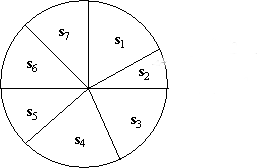
\includegraphics[scale=0.5]{img/rouletteSelect.png}
\end{center}
\item \textbf{Selekcja turniejowa} - wyłanianie osobników do procesu krzyżowania odbywa się poprzez pewną formę konkursu. Losowanych jest kilku uczestników (ich ilość jest jednym z parametrów algorytmu, wartość nominalna to 3), a wybierany jest ten spośród nich, który jest najlepiej przystosowany do środowiska. Zawodnicy w danym turnieju oczywiście muszą być różni, lecz po przeprowadzeniu wielu takich rozgrywek, najlepsi z nich powinni zostać wybierani najczęściej. Oznaczając $x, y, z$ jako wylosowanych do turnieju zawodników, $F(x), F(y), F(z)$ jako wartości ich funkcji oceny, to zwycięzcą zostanie najlepiej przystosowanych z nich:
\begin{center}
$F(winner) = \min(F(x), F(y), F(z))$
\end{center}
\end{enumerate}
\paragraph{}Selekcji poddane zostaną wszystkie osobniki, lecz w następnym etapie (krzyżowaniu) tylko te, które pozytywnie przejdą tę weryfikację.
\subsubsection{Krzyżowanie}
Proces ten polega na złączeniu w sposób losowy genotypu dwóch rodziców wybranych w poprzednim kroku w celu stworzenie potomka, który będzie dziedziczył po nich wszystkie cechy. W implementowanym rozwiązaniu, z danej pary rodziców tworzona jest dwójka dzieci będących początkowo kopiami swoich rodziców. Następnie część genotypu pierwszego dziecka jest zastępowana genotypem drugiego rodzica, a drugiemu dziecku wprowadzane są informacje dziedziczone po pierwszym rodzicu. Wykorzystując posiadaną wiedzę teoretyczną na temat tego etapu i próbując zastosować ją w kontekście posiadanej struktury planu zajęć, powstał opisany poniżej schemat postępowania.
\begin{enumerate}
\item Tworzymy kopie rodziców \emph{$dziecko_1$ = matka} oraz \emph{$dziecko_2$ = ojciec}
\item Losujemy kolejność kursów, których zajęcia zawarte u rodzica będą wprowadzane do drugiego dziecka w miejsce zajmowane w genotypie rodzica. W optymistycznym przypadku proces ten zostanie przerwany, gdy przeniesiemy połowę genotypu rodzica. Ponieważ nie zawsze uda się to osiągnąć pilnując jednocześnie, aby nie naruszone zostały twarde ograniczenia, proces ten będzie próbował zadaną ilość zamian osiągnąć iterując po wszystkich dostępnych zajęciach.
\item 
\begin{itemize}
\item Dla każdego przenoszonego zajęcia sprawdź, czy dane zajęcia i odpowiadające mu zajęcie u dziecka są identyczne. W takim wypadku nic nie rób i oznacz zamianę jako udaną.
\item Jeśli pomieszczenie jest już zajęte, oznacz operację jako nieudaną.
\item Jeśli pomieszczenie jest wolne i wprowadzenie zajęć w tym terminie nie narusza żadnych ograniczeń twardych, to oznacz operację jako pozytywną, w przeciwnym razie jako negatywną.
\end{itemize}
\end{enumerate}
\paragraph{}Cały opisany powyżej schemat zostaje powtórzony w analogiczny sposób dla drugiego dziecka, w którym zamienione miejscami zostają role rodziców. Umożliwia on losowe wymieszanie genów rodziców przy jednoczesnym zachowaniu ważności rozwiązania. Niestety nie zawsze udaje się znaleźć wystarczającą ilość miejsc dla wszystkich wprowadzanych genów tak, aby nie naruszało to ograniczeń twardych. Ilość materiału genetycznego każdego z rodziców powinna być jednakowa, jednak przeprowadzane testy wykazały, że próby przeprowadzenia pełnego krzyżowania wymagają często długiego wyszukiwania miejsca w genotypie dziecka dla wprowadzanego genu rodzica, co działa długo i nie daje dobrych wyników. Tworzone w ten sposób dzieci były gorzej oceniane niż ich rodzice. Dlatego proces ten został znacznie uproszczony i dopuszcza niepełne krzyżowania. Zmniejsza to różnorodność osobników (dzieci są bardziej podobne do swoich rodziców), ale skutkuje także tworzeniem lepiej przystosowanego potomstwa. Zabiegiem, który będzie zapobiegał zbytniemu upodobnieniu się osobników względem siebie będzie powiększanie współczynnika mutacji, który będzie różnicował coraz więcej osobników.
\paragraph{}Z każdej pary rodziców powstaje dwójka potomstwa. Zgodnie z zasadami ewolucji, gdzie przetrwać mogą tylko najlepiej przystosowani, do następnego pokolenia przejdzie lepsza połowa otrzymanych w tym procesie dzieci. Drugą połowę uzupełnią najlepiej przystosowane osobniki ze starszego pokolenia.
\subsubsection{Mutacja}
Podobnie jak w naturalnym procesie mutacji, tutaj też polega on na wprowadzeniu losowych zmian w powstałym potomku. Prawdopodobieństwo jego zajścia jest niewielkie (domyślnie 1\%), więc dotyczy pojedynczych genów u najwyżej kilku osobników i polegać będzie na zamianie ich miejscami. W typowych implementacjach algorytmu, w których rozwiązanie przechowywane jest w postaci ciągu bitów, mutacja sprowadza się najczęściej do negacji losowo wybranego bitu. W przypadku stosowanej struktury zajęć, etap ten polega na zamianie terminów i sal dwóch losowo wybranych zajęć. Ponieważ wprowadzenie takich zmian może skutkować naruszeniem ograniczeń koniecznych do spełnienia, należy temu zjawisku zapobiec. Dlatego w tym przypadku losowana jest para terminów i lekcji tak długo, aż zostanie wyłonione para, która nie powoduje naruszenia legalności rozwiązania. Istnieje także górne ograniczenie możliwych prób, którego ewentualne przekroczenie skutkować będzie zatrzymaniem procesu i brakiem mutacji w tym osobniku.
\subsubsection{Elityzm}
\paragraph{}Jest to zagadnienie związane po części z każdym etapem ewolucji rozwiązania. Zarówno krzyżowanie jak i mutacja ze względu na dużą losowość operacji, które wykonują, nie koniecznie muszą poprawiać wcześniej uzyskane rozwiązane. Pogorszenie wyniku w dłuższej perspektywie może okazać się pomocne, ponieważ umożliwiło inną, o wiele bardziej pozytywną zmianę, lecz z punktu widzenia całej populacji, lepiej jest unikać potencjalnego pogorszenia najlepszego wyniku. Dlatego wymienionym wyżej operacjom nie będziemy poddawać jednego (domyślnie) lub kilku najlepszych rozwiązań, aby nie utracić ich wyniku. Elityzmem nazywamy więc ochronę najlepszego rozwiązania przed możliwą regresją podczas operacji genetycznych.
\subsubsection{Implementacja}
\paragraph{}Przeprowadzane testy na większych zestawach danych wykazały, że wraz ze wzrostem ilości przeprowadzonych iteracji, osobniki upodabniają się do siebie i operacja krzyżowania nie zmienia wiele. Dlatego rola mutacji powinna wzrastać i z tego względu w każdej kolejnej epoce współczynnik mutacji zostaje zwiększany o 2\% dopóki współczynnik nie osiągnie wartości 50\%. Tak duża wartość jest jednak uzasadniona, ponieważ w przeciwnym wypadku po kilkuset iteracjach wszystkie osobniki stałyby się takie same.
\paragraph{}Opis struktury przetrzymującej plan zajęć oraz funkcja obliczająca wartość przystosowania osobnika pod kątem ograniczeń miękkich są takie same, jak w przypadku implementacji algorytmu \emph{Adaptive Tabu Search} i zostały one opisane w rozdziale \emph{4.1.5}. Oddzielnie stworzona została funkcja obliczająca karę za naruszanie ograniczeń twardych. Muszą one być o wiele większe, aby rozwiązania ich nie spełniające nie były w żadnym razie faworyzowane\cite{ga2003}. Różnica wielkości kar za ograniczenia miękkie oraz twarde jest rzędu $1:1000000$. W celu sprawdzenia wszystkich możliwych konfliktów powstały następujące funkcje, a wyliczane przez nie wartości sumują się do całkowitej kary za nieprzestrzeganie twardych ograniczeń.
\begin{itemize}
\item{countMissingLectures} - Za każde zajęcie, które nie zostało przypisane w rozkładzie zajęć nałóż karę w wysokości 1000000 punktów.
\item{countCurriculumConflicts} - Za każde zajęcia, które odbywają się w tym samym czasie co inne zajęcia należące do tego samego programu nauczania nałóż 1000000 punktów kary.
\item{countRoomOccupancy} - Za każde zajęcia, które odbywają się w danym momencie w tej samej sali co inne zajęcia nałóż karę w wysokości 1000000 punktów.
\item{countConstraintsList} - Wszystkim lekcjom, które odbywają się w chwili, gdy nauczyciel je prowadzący jest nieosiągalny, nadaj 1000000 punktów kary.
\item{countTeachersConflicts} - Za każdą dodatkową lekcję, którą nauczyciel ma prowadzić w tym samym czasie ukaraj 1000000 punktami kary.
\item{countRoomTypeViolations} - W przypadku danych szkolnych (opisanych w rozdziale \emph{6.1}), za każdą lekcję, która odbywa się w sali nieodpowiedniego typu nadaj karę 1000000 punktów.
\end{itemize}